\documentclass[a4paper]{article}
\usepackage[T1]{fontenc}
\usepackage[applemac]{inputenc}
\usepackage{ifthen}
\usepackage{xspace}
\usepackage{overpic}
\usepackage{garamath}
\usepackage{gillsans}
\usepackage{sectsty}
\allsectionsfont{\sffamily\bfseries}
% Num�ro de section dans la marge
\makeatletter
\def\@seccntformat#1{%
  \protect\makebox[0pt][r]{%
    \csname the#1\endcsname\quad
  }%
}
\makeatother

\usepackage[nohead,top=1cm,left=2.5cm,right=2cm,bottom=1cm,footskip=0.5cm]{geometry}
\usepackage{fancyhdr}
\pagestyle{fancy}
\fancyhead{}
\renewcommand{\headrulewidth}{0pt}
\lfoot{\textsf{\footnotesize BouMaton <\url{http://wwwsi.supelec.fr/fb/Development.html}>}}
\cfoot{\thepage}
\rfoot{\textsf{\footnotesize
  \href{mailto:Frederic.Boulanger@supelec.fr}{<Frederic.Boulanger@supelec.fr>}%
}}
\renewcommand{\footrulewidth}{0pt}

\usepackage[%
  pdfauthor={Fr�d�ric Boulanger},
  pdftitle={BouMaton manual},
  pdffitwindow,
  pdfstartview=XYZ,
  pdfpagemode=None
]{hyperref}

\newcommand{\signature}{%
  \vfill
  \begin{flushright}
    \href{mailto:Frederic.Boulanger@supelec.fr}{Fr�d�ric Boulanger},
    \the\year-\ifnum\the\month<10 0\fi\the\month-\ifnum\the\day<10 0\fi\the\day
  \end{flushright}
}
\AtEndDocument{\signature}

%\setlength{\parindent}{0pt}
%\setlength{\parskip}{1ex plus 0.5ex minus 0.5ex}

\newcommand{\bouVersion}{1.5\xspace}
\newcommand{\bouRelease}{2006-02-10\xspace}

\newcommand{\BouMaton}{\textsf{BouMaton}\xspace}
\newcommand{\filename}[1]{\textsf{#1}}
\newcommand{\menu}[1]{\textsf{\textbf{#1}}}
\newcommand{\picdim}[2]{#1\,\(\times\)\,#2}

\begin{document}
  \begin{center}
    \textsf{\textbf{\large BouMaton v\bouVersion, \bouRelease}}
    
    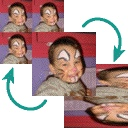
\includegraphics[scale=0.5]{icone}
    
    \href{mailto:Frederic.Boulanger@supelec.fr}{\textsf{Fr�d�ric Boulanger}}
  \end{center}
  
  
  \section{What is it?}
  \BouMaton is an application which computes two transforms on pictures:
  \begin{itemize}
    \item the \textbf{photomaton} transform dispatches the pixels of an 
    image toward its four corners, so that the result looks like four 
    identical sub-images, just like in the automatic photo machines you 
    use to get a picture for your ID card;
    
    \item the \textbf{boulanger} transform stretches the image 
    horizontally and then folds it so that it has the same size as the 
    original. This is similar to what a baker does when he kneads 
    bread, hence the name (boulanger is the french word for baker).
  \end{itemize}
  
  Both transforms retain all the information in the picture, so it is 
  always possible to retrieve the original image by applying the 
  reverse transform. Moreover, these transforms are periodic: After a 
  given number of iterations, the original image comes back.
  
  \BouMaton is able to apply these transforms and their reverse 
  transforms any number of times to a picture. It also computes the 
  periods of the transforms, and keeps a history of the transforms 
  so far applied. It can also save the resulting picture in JPEG format 
  if the necessary Java classes are available on your computer.
  
  \section{Quick start}
  \BouMaton is a Java application. On many platforms, double-clicking 
  the \filename{BouMaton.jar} file will launch it. In a command-line 
  shell, use \verb|java -jar BouMaton.jar| to launch \BouMaton. On 
  Mac~OS~X, double-click the \filename{BouMaton} application (but you 
  can also use the \filename{BouMaton.jar} archive or the command line).
  
  Once \BouMaton is running, select the \menu{Open...} item in the
  \menu{File} menu to open a picture.  The formats allowed for the
  pictures are those supported by the \filename{javax.imageio}
  package: at least jpeg, gif and png.
  
  Click the \menu{boulanger} or \menu{photomaton} button, or select
  the corresponding item in the \menu{Transforms} menu to apply a
  transform to the picture.  You can set the number of iterations
  (negative for reverse transforms) in the text field between the two
  buttons.
  
  If you started the computation of a large number of transforms on a 
  big picture and find that it takes too much time to complete, you can 
  interrupt the computation with the \menu{Interrupt} item of the 
  \menu{Transforms} menu.
  
  \section{A more detailed description}
  The main window of \BouMaton contains the following items:
  \begin{center}
    \sffamily
    \begin{overpic}[%
                    scale=.4,
                    %grid
                   ]{vue_generale}
      \put(-10,80){\makebox(0,0)[br]{picture view}}
      \put(-10,80){\vector(2,-1){25}}
      %
      \put(-10,20){\makebox(0,0)[br]{period computation progress}}
      \put(-10,20){\vector(3,-1){12}}
      %
      \put(-10,12){\makebox(0,0)[br]{boulanger transform button}}
      \put(-10,12){\vector(4,-1){12}}
      %
      \put(20,-2){\makebox(0,0)[tr]{picture dimensions}}
      \put(20,-2){\vector(1,2){8}}
      %
      \put(36,-2){\makebox(0,0)[tl]{number of iterations}}
      \put(35,-2){\vector(0,1){8}}
      %
      \put(80,12){\makebox(0,0)[bl]{photomaton transform button}}
      \put(80,12){\vector(-4,-1){10}}
      %
      \put(80,20){\makebox(0,0)[bl]{period of the photomaton transform}}
      \put(80,20){\vector(-3,-1){17}}
    \end{overpic}
  \end{center}

  \vspace{2cm}
  
  The picture view area displays the result of applying the transforms 
  to the picture. The period computation progress bar indicates that 
  the period of the boulanger transform of this picture is being 
  computed. When the computation is over, the progress bar is replaced 
  by the value of the period.
  
  The \menu{boulanger} and \menu{photomaton} buttons trigger the 
  computation of the corresponding transform, applied as many times as 
  indicated in the number of iterations text field.
  
  On the right side, you can see the period of the photomaton transform 
  for this picture (which is much faster to compute than the period of 
  the boulanger transform).
  
  In the following example, the view displays the result of the 
  photomaton transform applied once to the original picture, and the 
  program is computing 500 iterations of the photomaton transform.

  The picture view area does not display a live update of the picture
  as it is being transformed, since this would slow down the
  computation too much. The view is updated only when the computation
  of the transforms is over. This is why in this example, you see the
  result of the photomaton transform applied only once to the original
  picture, even if more than half of 500 requested iterations have
  already been computed.
  
  \begin{center}
    \sffamily
    \begin{overpic}[%
                    scale=.4,
                    %grid
                   ]{photomaton}
      \put(-10,12){\makebox(0,0)[br]{%
        \parbox{70\unitlength}{%
          disabled because a transform is being computed
        }%
      }}
      \put(-10,12){\vector(4,-1){12}}
      %
      \put(30,-17){\makebox(0,0)[t]{500 iterations requested}}
      \put(30,-15){\vector(1,4){5}}
      %
      \put(80,12){\makebox(0,0)[bl]{%
        \parbox{70\unitlength}{%
          disabled because a transform is being computed
        }%
      }}
      \put(80,15){\vector(-4,-1){17}}
      %
      \put(80,0){\makebox(0,0)[tl]{%
        \parbox{70\unitlength}{%
          progress of the computation of the 500 iterations of the 
          photomaton transform
        }%
      }}
      \put(80,0){\vector(-4,1){14}}
    \end{overpic}
  \end{center}
  
  \vspace{2cm}
  
  The behavior for the boulanger transform is similar. In the
  following example, the view displays the result of the boulanger
  transform applied once to the original picture, and the program is
  computing 500 iterations of the boulanger transform:
  \begin{center}
    \sffamily
    \begin{overpic}[%
                    scale=.4,
                    %grid
                   ]{boulanger}
      \put(-10,12){\makebox(0,0)[br]{%
        \parbox{70\unitlength}{%
          disabled because a transform is being computed
        }%
      }}
      \put(-10,12){\vector(4,-1){12}}
      %
      \put(30,-17){\makebox(0,0)[t]{500 iterations requested}}
      \put(30,-15){\vector(1,4){5}}
      %
      \put(80,12){\makebox(0,0)[bl]{%
        \parbox{70\unitlength}{%
          disabled because a transform is being computed
        }%
      }}
      \put(80,15){\vector(-4,-1){17}}
      %
      \put(-10,0){\makebox(0,0)[tr]{%
        \parbox{70\unitlength}{%
          progress of the computation of the 500 iterations of the 
          boulanger transform
        }%
      }}
      \put(-10,0){\vector(4,1){10}}
    \end{overpic}
  \end{center}
  
  \vspace{2cm}

  \section{Saving pictures}
  Since version 1.4, \BouMaton requires at least Java~1.4 to run, but
  is able to save pictures in either JPEG or PNG format.
  
  The JPEG format yields smaller files for photographs but ignores details
  that are considered less important due to the way human eyes work.
  When you save a file in JPEG format, you can choose how much
  information will be discarded by setting the quality of the saved
  picture.  The setting ranges from 0 (very aggressive compression,
  small file, very low quality), to 100 (weakest compression, large
  file, but high quality).  To help you in this choice, \BouMaton can
  compute the estimated size of the file with the current quality
  setting if you click the \menu{Compute file size} button in this
  dialog.  If the estimated file size is lower than the size of the
  original JPEG file, your setting is too low.  If it is much higher,
  your setting is too high.  However, since the transforms make the
  picture more and more complex, it is normal that the estimated size
  grows when you save successively transformed pictures with the same
  quality setting.
  
  The PNG format discards no information. Therefore, pictures saved 
  in this format tend to use much more disk space than pictures saved 
  in the JPEG format. However, PNG uses a lossless compression 
  algorithm that is more efficient than JPEG compression for pictures 
  that contain only lines and large areas of a uniform color. Since 
  the PNG format does not discard information, you should use it to 
  save transformed pictures that you want to restore to their 
  original form later by applying inverse transforms.
  
%   \section{Saving pictures as JPEG}
%   If \BouMaton found the necessary classes on your computer, the
%   \menu{Save...} item in the \menu{File} menu is enabled and allows
%   you to save the marvelous results of your playing with \BouMaton.
%   The only supported format for saving pictures is JPEG. This format
%   reduces the size of the picture file by ignoring details which are
%   considered less important due to the way human eyes work. When you
%   save a picture to a file, \BouMaton displays a dialog to let you set
%   how aggressive you want JPEG compression to be. The setting ranges
%   from 0 (very aggressive compression, small file, very low quality),
%   to 100 (weakest compression, large file, but high quality). To help
%   you in this choice, \BouMaton can compute the estimated size of
%   the file with the current quality setting if you click the
%   \menu{Compute file size} button in this dialog. If the estimated
%   file size is lower than the size of the original JPEG file, your
%   setting is too low. If it is much higher, your setting is too high.
%   However, since the transforms make the picture more and more
%   complex, it is normal that the estimated size grows when you save
%   successively transformed pictures with the same quality setting.
  
  \section{History of the transforms}
  \BouMaton keeps track of all the transforms you have applied to a 
  picture. You can view this history by selecting the \menu{Show history} 
  item in the \menu{Transforms} menu:
  \begin{center}
    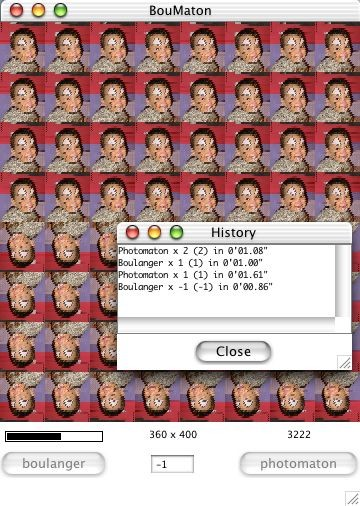
\includegraphics[scale=0.4]{history}
  \end{center}
  Consecutive identical transforms are merged in the history, so that 
  two successive photomaton transforms make only one entry in the 
  history. Each entry shows the nature of the transform, the number of 
  iterations, the effective number of iterations computed, and the 
  time used to compute them. The effective number of iterations may be 
  less than the required number since computing 3225 iterations of a 
  transform which has a period of 3222 for the picture is exactly the 
  same as computing only 3 iterations (but takes more time!). With the 
  same period, if you ask for 3200 iterations, \BouMaton will compute 
  22 iterations of the reverse transform since this is much faster.
  
  You can always revert to the original picture by choosing the 
  \menu{Revert} item of the \menu{File} menu. This also clears the history.
  
  \section{Information about the transforms}
  While computing the periods of the transforms, \BouMaton gathers 
  information about the period of individual pixels. During successive 
  transforms, each pixel follows an orbit (it goes from place to place 
  in the picture) and may come back to its original position well 
  before the whole picture is restored. The period of the transform for 
  the picture is the smallest number of iterations such that each pixel 
  has completed a whole number of turns on its own orbit.
  
  It may happen that after a given number of iterations of a 
  transform, many pixels are back to their original position, so that 
  the original image seems to appear again in the otherwise 
  random-looking set of pixels.
  
  Selecting the \menu{Show info} item of the \menu{Transform} menu 
  will display all the information gathered so far about both transforms. 
  Information about the boulanger transform is quite long to compute 
  and won't be displayed until the period of the transform is computed.
  
  \begin{center}
    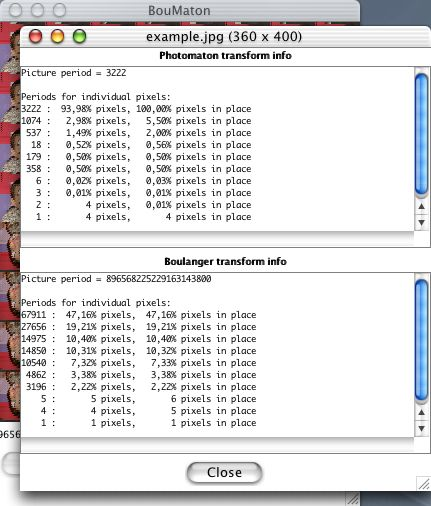
\includegraphics[scale=0.4]{info}
  \end{center}
  This example shows the information for a \picdim{360}{400} picture 
  (the periods depend only on the geometry of the picture). We can see 
  that the period of the boulanger transform is quite big, but that 
  after 67911 iterations, 47.16\,\% of the pixels are back to their 
  original position.
  
  \section{Examples}
  The following series of pictures show the evolution of an image for
  both transforms, from the original through pictures where all
  information seems to be lost and others where ghosts of the original 
  appear, and finally back to the original.
  
  \subsection{Iterations of the photomaton transform}

  {\sffamily\small
  \begin{tabular}{@{}*5{p{0.18\textwidth}}@{}}
    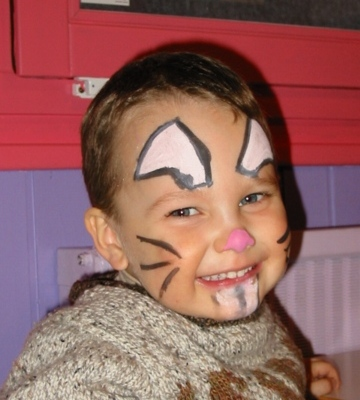
\includegraphics[width=\linewidth]{example}
    &
    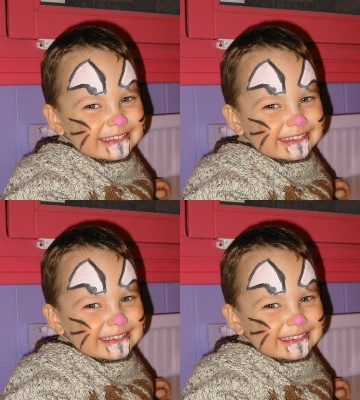
\includegraphics[width=\linewidth]{example_p1}
    &
    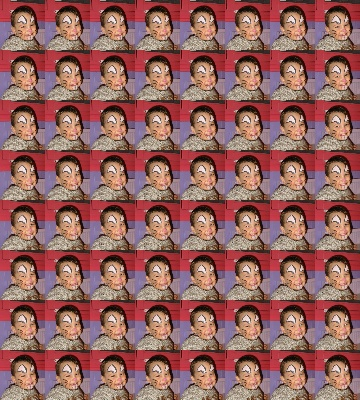
\includegraphics[width=\linewidth]{example_p3}
    &
    
\includegraphics[width=\linewidth]{example_p8}
    &
    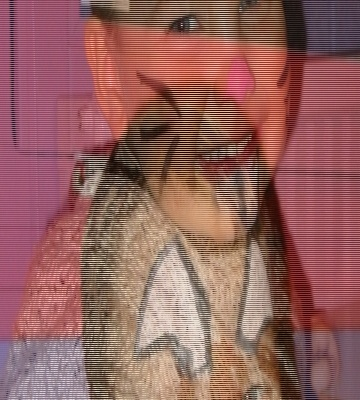
\includegraphics[width=\linewidth]{example_p179}
    \\
      original picture
    & after one iteration
    & after 3 iterations
    & after 8 iterations
    & something appears after 179 iterations
    \\[10pt]
    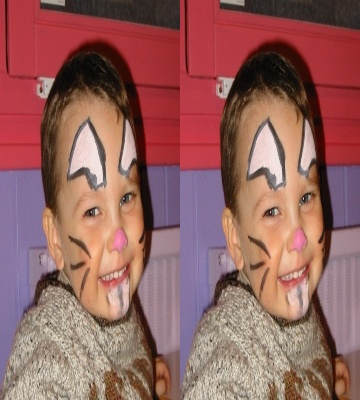
\includegraphics[width=\linewidth]{example_p180}
    &
    
\includegraphics[width=\linewidth]{example_p_6}
    &
    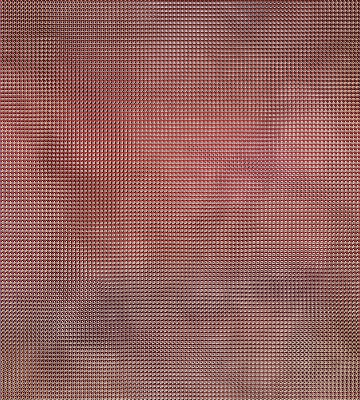
\includegraphics[width=\linewidth]{example_p_2}
    &
    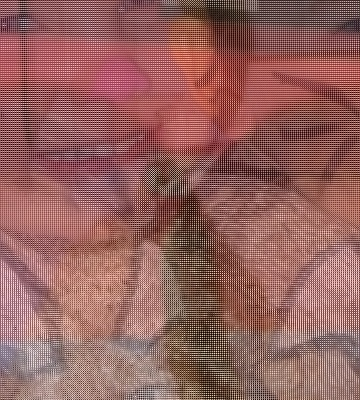
\includegraphics[width=\linewidth]{example_p_1}
    &
    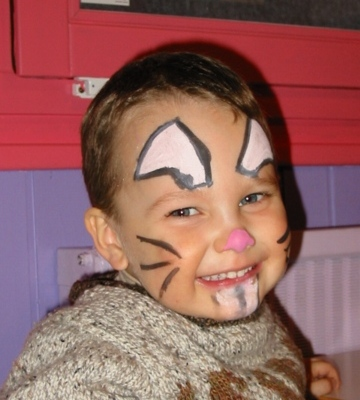
\includegraphics[width=\linewidth]{example}
    \\
      close to the original after 180 iterations
    & 6 iterations before the original
    & 2 iterations before the original
    & 1 iteration before the original
    & back to the original after 3222 iterations
  \end{tabular}
  }
  
  \subsection{Iterations of the boulanger transform}
  {\sffamily\small
  \begin{tabular}{@{}*5{p{0.18\textwidth}}@{}}
    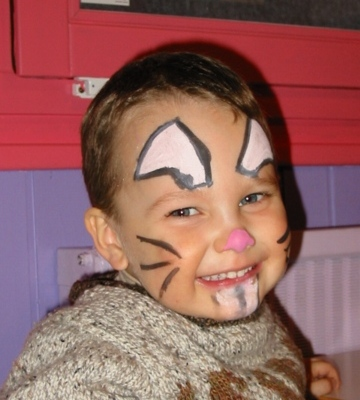
\includegraphics[width=\linewidth]{example}
    &
    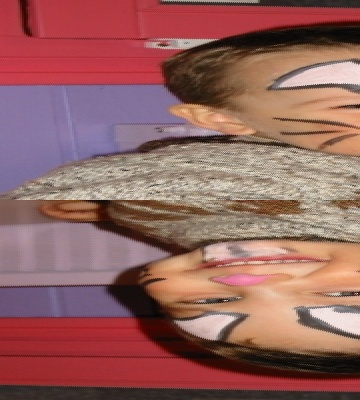
\includegraphics[width=\linewidth]{example_b1}
    &
    
\includegraphics[width=\linewidth]{example_b4}
    &
    
\includegraphics[width=\linewidth]{example_b20}
    &
    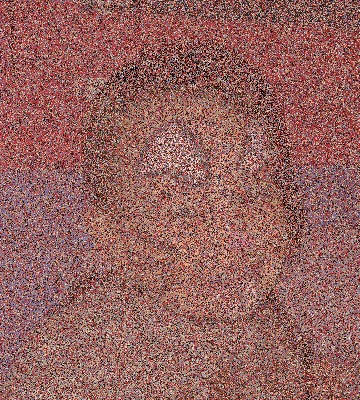
\includegraphics[width=\linewidth]{example_b27656}
    \\
      original picture
    & after one iteration
    & after 4 iterations
    & after 20 iterations
    & 19.2\% pixels are in place after 27656 iterations
    \\[10pt]
    
\includegraphics[width=\linewidth]{example_b67911}
    &
    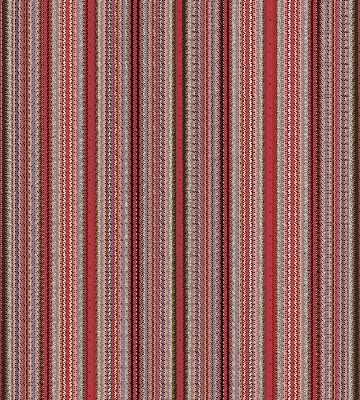
\includegraphics[width=\linewidth]{example_b_6}
    &
    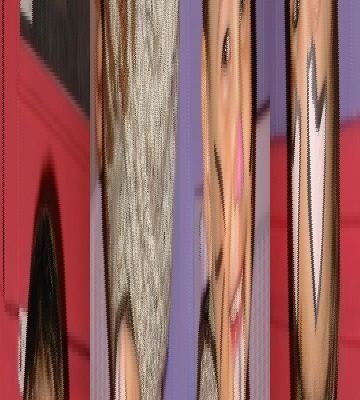
\includegraphics[width=\linewidth]{example_b_2}
    &
    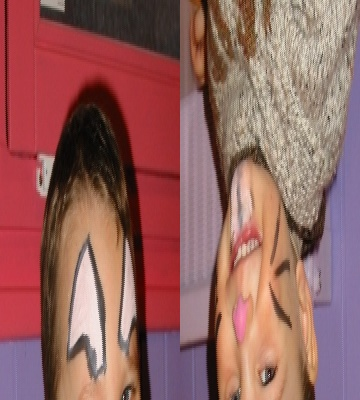
\includegraphics[width=\linewidth]{example_b_1}
    &
    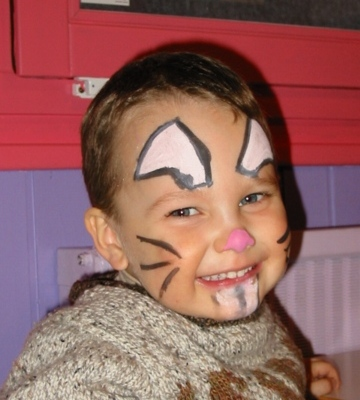
\includegraphics[width=\linewidth]{example}
    \\
      47.2\% pixels are in place after 67911 iterations
    & 6 iterations before the original
    & 2 iterations before the original
    & 1 iteration before the original
    & back to the original after {\tiny 896568225229163143800} iterations
  \end{tabular}
  }
  
  \section{Licence}
  \newlength{\savedindent}
  \setlength{\savedindent}{\parindent}
  \setlength{\parindent}{0pt}
  \newlength{\savedskip}
  \setlength{\savedskip}{\parskip}
  \setlength{\parskip}{1ex}
  
  \BouMaton is copyright Fr�d�ric Boulanger 1997-2006, all rights 
  reserved.
  
  \BouMaton and its source code may be freely redistributed as long as
  it is not modified and that the distribution includes this 
  documentation. Translations of the application and the documentation 
  are allowed, but the original versions (see \ref{sec:tech-details} 
  below) must always be included in the distribution.
  
  \BouMaton is distributed ``as is'' with absolutely no warranties 
  with respect to its quality, accuracy or fitness for a particular 
  purpose.
  
  Parts of the source code of \BouMaton may be freely used in other 
  applications as long as this use is acknowledged in the documentation 
  and in the application, for instance in the ``about box'' or in the 
  initial prompt if the application has no graphical interface.
  
  The name ``\BouMaton'' cannot be used for modified versions of 
  \BouMaton, and the author of the modified version must make clear 
  that I am not the primary author of his application.
  
  \setlength{\parindent}{\savedindent}
  \setlength{\parskip}{\savedskip}
  
  \section{History of \BouMaton}
  Everything began with an article by Jean-Paul Delahaye and Philippe 
  Mathieu in the December 1997 issue (\#\,242) of ``Pour la Science'', the 
  French edition of Scientific American. This article described the 
  photomaton and the boulanger transforms, and I started coding these 
  transforms in C. To avoid writing a real application, I used the 
  plug-in API of GraphicConverter, a very smart application for Mac~OS 
  which reads and writes almost any picture file 
  (\url{http://www.lemkesoft.com/us_gcabout.html}). The result was two 
  plug-ins named \filename{PhotoMaton} and \filename{Boulanger} 
  (\url{http://wwwsi.supelec.fr/fb/Development.html#progs}).
  
  GraphicConverter switched to Carbon when Mac~OS~X appeared, and 
  instead of converting my plug-ins to Carbon, I decided to write a 
  Java application combining the functionalities of both plug-ins. 
  This allowed me to keep a history of the transforms applied to a 
  picture and to display information concerning the period for the whole 
  image and for individual pixels. Using BigIntegers, I was able to 
  fix a bug in the computation of the period of the boulanger 
  transform which often overflows unsigned long integers.
  
  The result is \BouMaton, and I hope that the users of the 
  GraphicConverter plug-ins will appreciate it, and that Windows and 
  Unix users will benefit from the ``write once, execute anywhere'' 
  Java motto.
  
  \medskip
  
  \noindent Version 1.0 is the first public release of \BouMaton.
  \par\smallskip
  \noindent Version 1.1 fixes a picture update issue.
  \par\smallskip
  \noindent Version 1.2 improves low-memory conditions handling and
  adds a dialog to set the JPEG compression quality when saving a picture.
  \par\smallskip
  \noindent Version 1.3 uses a new algorithm to compute the period of 
  the boulanger transform more quickly.
  \par\smallskip
  \noindent Version 1.4 uses the javax.imageio package and adds
  support for saving pictures in PNG.
  \par\smallskip
  \noindent Version 1.5 fixes a problem with reading PNG images.
  
  \section{Technical details\label{sec:tech-details}}
  This section explains technical details of \BouMaton and may be 
  ignored safely by casual users.
  
  \subsection{Translations of \BouMaton}
  The manual of \BouMaton is written in \LaTeX. You can start from the 
  English or French versions of the manual and translate it into another 
  language. You should then identify yourself as the translator.
  
  The strings used in \BouMaton can also be translated into other 
  languages. The jar file contains a 
  \filename{BouMatonStrings.properties} file which is for the English 
  (default) version. The \filename{BouMatonStrings\_fr.properties} 
  file is used when the default locale specifies the French language. 
  If you want to translate \BouMaton into another language, you have 
  to write a \filename{BouMatonStrings\_<lang>.properties} file, where 
  \filename{<lang>} is the locale code for your language (for instance 
  \filename{de} for German, \filename{it} for Italian and so on). The 
  easiest way to write this file is to start with a copy of one of 
  files I wrote for English and for French, and to translate each 
  phrase which is on the right side of the first ``='' sign on a line.
  The file must be added to the jar file for the new strings to be used 
  when the corresponding locale is active.
  
  If you write a translation for your language, please send me the file 
  so that I can put it in a future release of \BouMaton. A translated 
  manual would be appreciated too.
  
  \subsection{The boulanger transform}
  The stretching of the picture in the boulanger transform 
  is done by interleaving the pixels of odd lines with the pixels 
  of even lines. The folding is done by cutting the stretched picture 
  at its original width, and by rotating the right part around its 
  lower left corner, as shown below for a \picdim{4}{4} picture:
  
  \begin{center}
    \newcommand{\pixbox}[2]{\makebox(1,1){\textsf{\scriptsize(#1,#2)}}}
    \newcounter{pixx}
    \newcounter{pixy}
    \newcounter{pixnum}
    \newcommand{\dopixbox}[2]{%
      \put(\thepixx,\thepixy){\pixbox{#1}{#2}}%
      \stepcounter{pixx}%
      \bouline{\thepixy}{\thepixx}{\thepixnum}%
    }
    \newcommand{\bouline}[3]{%
      \let\next=\relax
      \ifnum#2<#3
        \setcounter{pixy}{#1}%
        \setcounter{pixx}{#2}%
        \setcounter{pixnum}{#3}%
        \let\next=\dopixbox
      \fi
      \next
    }
    \setlength{\unitlength}{0.5cm}
    \begin{picture}(22,4)
      \put(0,0){\framebox(4,4){}}
      \multiput(0,1)(0,1){3}{\line(1,0){4}}
      \multiput(1,0)(1,0){3}{\line(0,1){4}}
      \bouline{3}{0}{4} 0 0  0 1  0 2  0 3
      \bouline{2}{0}{4} 1 0  1 1  1 2  1 3
      \bouline{1}{0}{4} 2 0  2 1  2 2  2 3
      \bouline{0}{0}{4} 3 0  3 1  3 2  3 3
      %%
      \put(5,2){\vector(1,0){1}}
      %%
      \qbezier(0.5,3.9)(6,5)(7.5,2.9)\put(7.5,2.9){\circle*{0.12}}
      \qbezier(0.5,2.1)(6,1)(8.5,2.1)\put(8.5,2.1){\circle*{0.12}}
      %%
      \put(7,1){\framebox(8,2){}}
      \put(7,2){\line(1,0){8}}
      \multiput(8,1)(1,0){7}{\line(0,1){2}}
      \bouline{2}{7}{15} 0 0  1 0  0 1  1 1  0 2  1 2  0 3  1 3
      \bouline{1}{7}{15} 2 0  3 0  2 1  3 1  2 2  3 2  2 3  3 3
      %%
      \put(16,2){\vector(1,0){1}}
      %%
      \put(11,1){\circle*{0.25}}
      \put(11,0.9){\oval(3.5,3)[br]}
      \put(11,-0.6){\vector(-1,0){0.5}}     
      %%
      \put(18,0){\framebox(4,4){}}
      \multiput(18,1)(0,1){3}{\line(1,0){4}}
      \multiput(19,0)(1,0){3}{\line(0,1){4}}
      \bouline{3}{18}{22} 0 0  1 0  0 1  1 1
      \bouline{2}{18}{22} 2 0  3 0  2 1  3 1
      \bouline{1}{18}{22} 3 3  2 3  3 2  2 2
      \bouline{0}{18}{22} 1 3  0 3  1 2  0 2
      %%
      \put(22,2){\circle*{0.25}}
      \put(22.2,2){\oval(3,3)[br]}\put(22.2,0.5){\vector(-1,0){0.1}}
    \end{picture}
  \end{center}

  There is no loss of information in this transform, and after a
  number of iterations, the original image comes back. However, I
  don't know of a formula to compute this number for all pictures. For
  a \(2^m\) by \(2^m\) image, the original comes back after \(2m+1\)
  iterations. For a \(2^m\) by \(2^n\) image, you must wait for
  \((2m+1)(2n+1)+1\) iterations.

  To compute the period of the transform for a given
  picture, \BouMaton computes the period \(P(x,y)\) of each pixel
  of the picture (the number of iterations after which the pixel comes
  back to its original location).  The period \(P\) of the picture is the
  smallest common multiple of all \(P(x,y)\).  This computation may
  be quite long, and \BouMaton uses a separate thread to make it. 
  Since the period may be very large (896568225229163143800 for a 
  \picdim{360}{400} picture), \BouMaton uses BigIntegers to compute 
  the smallest common multiple of the pixel periods.
  
  Since version 1.3, \BouMaton uses a new algorithm to compute this 
  period much more quickly than before. When we are computing the 
  period of a given pixel, we find all the other pixels that belong to 
  its orbit. All those pixels have the same period since they belong 
  to the same orbit, therefore, there is no need to compute their 
  period again. Since there are generally few orbits in a picture, 
  the number of \(P(x,y)\) periods to compute is dramatically reduced 
  when using this optimization, and the period of the boulanger 
  transform is now computed as fast as the period of the photomaton 
  transform.
  
  \subsection{The photomaton transform}
  The photomaton transform splits a picture into what looks like four 
  identical copies of the original. However, the four copies are not 
  identical, and the four sub-pictures are obtained by selecting one 
  pixel in each \picdim{4}{4} square of the original image, as shown 
  in the following illustration for a \picdim{8}{8} image:
  \begin{center}
    \newcommand{\pixbox}[2]{\makebox(1,1){\textsf{\scriptsize(#1,#2)}}}
%     \newcounter{pixx}
%     \newcounter{pixy}
%     \newcounter{pixnum}
    \newcommand{\dopixbox}[2]{%
      \put(\thepixx,\thepixy){\pixbox{#1}{#2}}%
      \stepcounter{pixx}%
      \pholine{\thepixy}{\thepixx}{\thepixnum}%
    }
    \newcommand{\pholine}[3]{%
      \let\next=\relax
      \ifnum#2<#3
        \setcounter{pixy}{#1}%
        \setcounter{pixx}{#2}%
        \setcounter{pixnum}{#3}%
        \let\next=\dopixbox
      \fi
      \next
    }
    \setlength{\unitlength}{0.5cm}
    \begin{picture}(19,9)
      \put(0,0){\framebox(8,8){}}
      \multiput(1,0)(1,0){7}{\line(0,1){8}}
      \multiput(0,1)(0,1){7}{\line(1,0){8}}
      \pholine{7}{0}{8} 0 0  0 1  0 2  0 3  0 4  0 5  0 6  0 7
      \pholine{6}{0}{8} 1 0  1 1  1 2  1 3  1 4  1 5  1 6  1 7
      \pholine{5}{0}{8} 2 0  2 1  2 2  2 3  2 4  2 5  2 6  2 7
      \pholine{4}{0}{8} 3 0  3 1  3 2  3 3  3 4  3 5  3 6  3 7
      \pholine{3}{0}{8} 4 0  4 1  4 2  4 3  4 4  4 5  4 6  4 7
      \pholine{2}{0}{8} 5 0  5 1  5 2  5 3  5 4  5 5  5 6  5 7
      \pholine{1}{0}{8} 6 0  6 1  6 2  6 3  6 4  6 5  6 6  6 7
      \pholine{0}{0}{8} 7 0  7 1  7 2  7 3  7 4  7 5  7 6  7 7
      %
      \put(9,4){\vector(1,0){1}}
      %
      \put(11,0){\framebox(8,8){}}
      \multiput(12,0)(1,0){7}{\line(0,1){8}}
      \multiput(11,1)(0,1){7}{\line(1,0){8}}
      \pholine{7}{11}{19} 0 0  0 2  0 4  0 6  0 1  0 3  0 5  0 7
      \pholine{6}{11}{19} 2 0  2 2  2 4  2 6  2 1  2 3  2 5  2 7
      \pholine{5}{11}{19} 4 0  4 2  4 4  4 6  4 1  4 3  4 5  4 7
      \pholine{4}{11}{19} 6 0  6 2  6 4  6 6  6 1  6 3  6 5  6 7
      \pholine{3}{11}{19} 1 0  1 2  1 4  1 6  1 1  1 3  1 5  1 7
      \pholine{2}{11}{19} 3 0  3 2  3 4  3 6  3 1  3 3  3 5  3 7
      \pholine{1}{11}{19} 5 0  5 2  5 4  5 6  5 1  5 3  5 5  5 7
      \pholine{0}{11}{19} 7 0  7 2  7 4  7 6  7 1  7 3  7 5  7 7
      %%
      \qbezier(0.5,7.9)(8,9)(11.5,7.9)\put(11.5,7.9){\circle*{0.12}}
      \qbezier(1.5,7.9)(9,10)(15.5,7.9)\put(15.5,7.9){\circle*{0.12}}
      \qbezier(0.5,6.1)(8,3)(11.5,3.1)\put(11.5,3.1){\circle*{0.12}}
      \qbezier(1.5,6.1)(8,1)(15.5,3.1)\put(15.5,3.1){\circle*{0.12}}
      %%
      \thicklines
      \put(11,4){\line(1,0){8}}
      \put(15,0){\line(0,1){8}}
    \end{picture}
  \end{center}
  
  Since no information is lost in this transform, and the number of
  permutations of the pixels is finite, the original image comes back
  after a number of iterations. I don't know of a formula to compute
  the period of the photomaton transform for all pictures. For a
  \(2^m\) by \(2^n\) picture, the period is the smallest common
  multiple of \(m\) and \(n\), so a \picdim{512}{512} image will come
  back after 9 iterations, while a \picdim{128}{256} one has a period
  of 56.
  
  However, the period of the photomaton transform is much easier to
  compute than the period of the boulanger transform because the
  period of the \(x\) coordinate of all pixels with the same \(x\)
  coordinate is the same (all pixels on a same vertical line are back
  on this line at the same time), and the period of the \(y\)
  coordinate of all pixels with the same \(y\) coordinate is the same 
  (all pixels on a horizontal line are back on this line at the same 
  time).
  The period \(P(x,y)\) for a given pixel is the smallest common
  multiple of the period for \(x\) and the period for \(y\). The
  period for the whole image is the smallest common multiple of all
  \(P(x,y)\).
  
  \subsection{Optimizations}
  When the period \(P\) of a transform has been computed, \BouMaton
  uses it to optimize the computation of \(n\) iterations of the
  transform: it computes only \(n \bmod P\) iterations.  If \(n \bmod
  P\) is closer to \(P\) than to 0, it computes only \(P - (n \bmod
  P)\) iterations of the reverse transform.  Moreover, for each pixel
  in the image, \BouMaton uses the period for that pixel in the same
  way to optimize the number of iterations to compute.
  
  \subsection{Saving transformed image as JPEG}
  \BouMaton allows to save transformed pictures in either JPEG or PNG
  format.  We have seen that both transforms keep all the information
  that was in the original picture, but since JPEG compression is
  lossy, saving a transformed picture in JPEG and loading it later in
  \BouMaton to apply the reverse transforms will not yield an exact
  copy of the original picture.  The global aspect of the picture will
  be preserved, but colors may be washed out since JPEG compression
  will have discarded information which seemed not to be critical in
  the transformed image. There is no such problem with the PNG format 
  since it does not discard any information. 
\end{document}
